 % ****** Start of file apssamp.tex ****** %
 %   This file is part of the APS files in the REVTeX 4 distribution. %   Version 4.0 of REVTeX, August 2001 %
 %   Copyright (c) 2001 The American Physical Society. %
 %   See the REVTeX 4 README file for restrictions and more information. %
 % TeX'ing this file requires that you have AMS-LaTeX 2.0 installed %
 % as well as the rest of the prerequisites for REVTeX 4.0 %
 % See the REVTeX 4 README file % It also requires runninzzzzg BibTeX.

\documentclass[twocolumn,showpacs,preprintnumbers,amsmath,amssymb]{revtex4}
%\documentclass[preprint,showpacs,preprintnumbers,amsmath,amssymb]{revtex4}

% Some other (several out of many) possibilities %\documentclass[preprint,aps]{revtex4}
%\documentclass[preprint,aps,draft]{revtex4}
%%\documentclass[prb]{revtex4}% Physical Review B
\usepackage{amsmath}
\usepackage{graphicx}% Include figure files
\usepackage{dcolumn}% Align table columns on decimal point
\usepackage{bm}% bold math
\usepackage{braket}
%\nofiles

\begin{document}

\preprint{APS/123-QED}

\title{A Phenomenological Model of Photoinduced\\ Surface Relief Formation in Arsenic Sulfide}% Force line breaks with \\

\author{Daniel Recht}
% \altaffiliation[Also at ]{Physics Department, XYZ University.}%Lines break automatically or can be forced with \\
\author{Craig Arnold}%
 \email{cbarnold@princeton.edu}
\affiliation{Princeton University }%
\date{\today}%z

\begin{abstract}
An article usually includes an abstract, a concise summary of the work covered at length
in the main body of the article. It is used for secondary publications and for
information retrieval purposes. Valid PACS numbers may be entered using the
\verb+\pacs{#1}+ command.
\end{abstract}

\pacs{Valid PACS appear here}% PACS, the Physics and Astronomy
%\keywords{Suggested keywords}%Use showkeys class option if keyword
\maketitle

\section{\label{sec:intro}Introduction}

It has long been known that photoinduced processes can lead to mass transport in a
variety of systems generating surface relief.  A variety of systems exhibit photoinduced
expansion and or contraction.


 While it has long been known that thin arsenic sulfide (As$_{2}$S$_{3}$) films
expand when exposed to above-bandgap light, the mechanism by which this occurs is still
open to debate \cite{igo74, hegedus, ganjoo}. Two fairly recent discoveries reveal that
the situation is far more complex than it first appears. First, in 1994 Hisakuni and
Tanaka found that exposure of As$_{2}$S$_{3}$ to laser light could induce expansions a
full order of magnitude greater than had previously been observed even for very low
intensities \cite{hisakuni94}. In order to explain this athermal effect, Hisakuni and
Tanaka proposed and soon verified that As$_{2}$S$_{3}$ displays photoinduced fluidity
\cite{hisakuni95}.

The second major development was the discovery by Saliminia et al. (hereafter Saliminia)
in 2000 that thin films of As$_{2}$S$_{3}$ will respond to the polarization of a Gaussian
beam to which they are exposed by undergoing mass transport along the polarization vector
\cite{saliminia}. Salminia's group also exposed films to several interference patterns
with intensity gradients and to others with modulated polarization and observed the
formation of surface relief gratings of a size comparable to the ``giant'' photoexpansion
in both cases. Although surface relief gratings had been observed in the past, those
early studies reported much smaller features \cite{galstyan}. In 2005, Asatryan et al.
(hereafter Asatryan) repeated Saliminia's experiment at much lower intensities and found
a similar result for polarization modulation but did not observe grating formation under
intensity contrast \cite{asatryan05}. Saliminia and Asatryan's results are summarized in
table \ref{tab:comparison}.

\begin{table}
\begin{ruledtabular}
\begin{tabular}{l l l l }
\multicolumn{2}{c}{\textbf{Illumination Conditions}}&\multicolumn{2}{c}{\textbf{Surface Relief}}\\
\hline
\textbf{Polarization of}&\textbf{Modulated}&\textbf{Seen by}&\textbf{Seen by}\\
\textbf{Initial Beams}& \textbf{Quantity}&\textbf{Saliminia}&\textbf{Asatryan}\\
\hline
s-s &Intensity&$\frac{1}{2}$ p-p    &   None\\
p-p &Intensity&Major    &   None\\
s-p&Polarization&$\frac{3}{4}$ p-p&None\\
45-135&Polarization&$\approx$ p-p&Major\\
RCP-LCP&Polarization&Not tested&Major\\
\end{tabular}
\end{ruledtabular}
\caption{A comparison of the observations reported by Saliminia and Asatryan concerning
which illumination conditions lead to the formation of surface relief gratings. See
Figure \ref{fig:setup} for a definition of s and p polarization in terms of the film's
natural coordinate system. The angles in 45-135 polarization are measured above the
positive $x$ (s) axis. LCP and RCP refer respectively to left and right circular
polarization.} \label{tab:comparison}
\end{table}

After addressing and explaining the apparent contradictions between Saliminia and
Asatryan's data, this paper presents a phenomenological model describing surface relief
formation as incompressible flow driven by a photoinduced pressure and damped by surface
tension. Despite the fact that both polarization and intensity modulation may lead to
this effect, a single expression for the photoinduced pressure, derived without any
assumptions about the microstructure of As$_2$S$_3$, is shown to be sufficient. Finally,
results of the model are considered.

\begin{figure}
 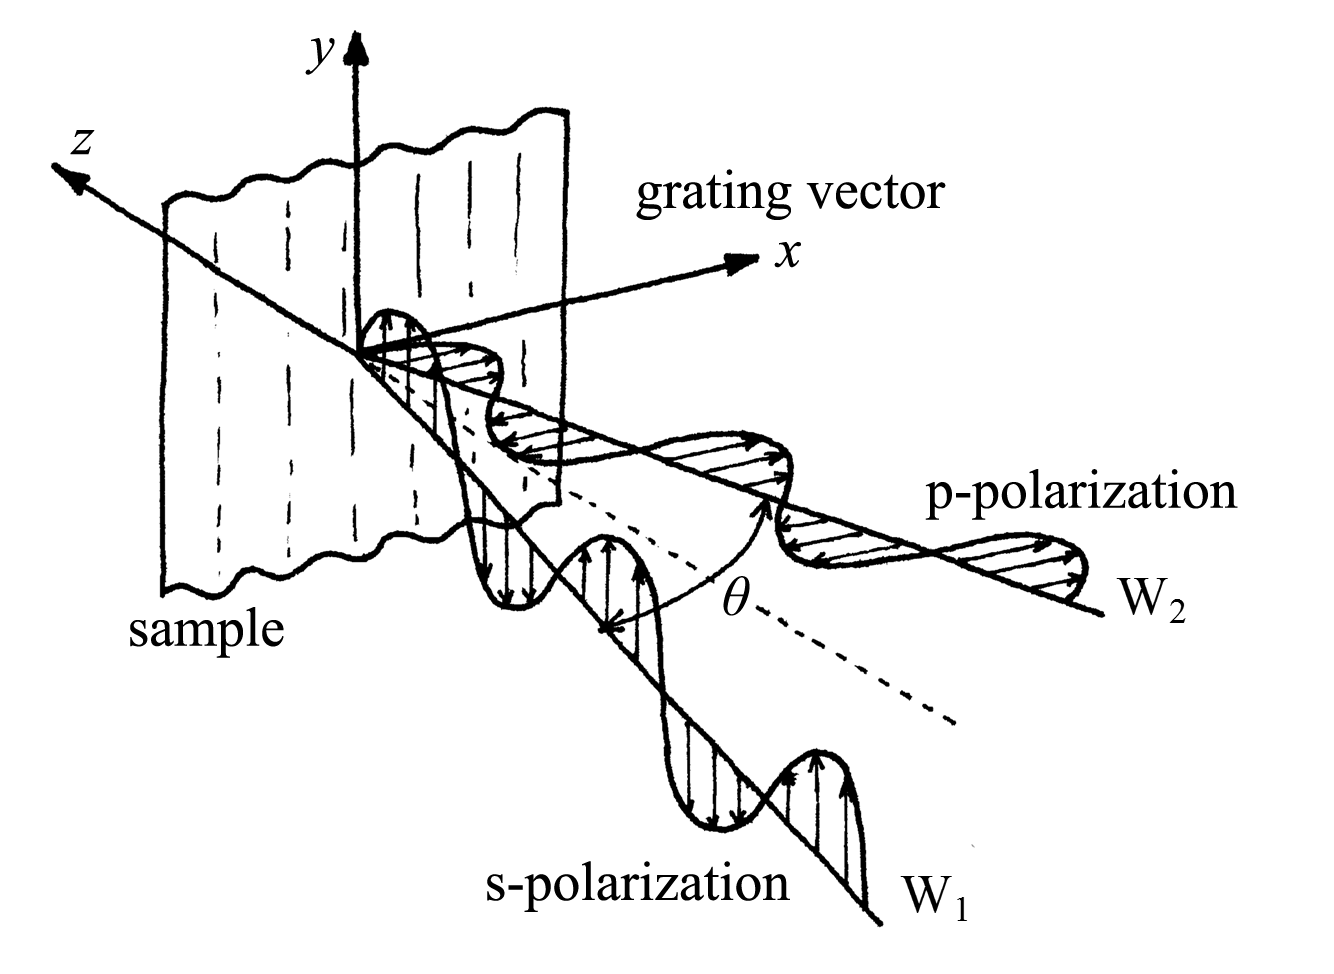
\includegraphics[width=1.75in]{figure/sppic.png}
 \caption{Schematic diagram of the experimental setup used by Saliminia and Asatryan.
   Two beams, W1 and W2, interfere on the surface of a thin film of As$_{2}$S$_{3}$ leading
   to the pictured definitions of the coordinate system and polarization directions.}
 \label{fig:setup}
\end{figure}

\section{The Model}

\subsection{Reconciling Saliminia and Asatryan}
The most important issue raised by Table \ref{tab:comparison} is that Saliminia observed
grating formation in response to intensity modulation while Asatryan did not. Naturally,
one must look to their procedures for an answer. The most striking difference between
their two studies is the intensity of the light used to illuminate the As$_{2}$S$_{3}$
films. While Saliminia used an intensity of $105$ W/cm$^{2}$, Asatryan used just $350$
mW/cm$^{2}$. One might be tempted to suggest that 1) photoinduced fluidity is a necessary
precursor to mass transport and 2) Asatryan's intensity was insufficient to bring this
about. Unfortunately for this explanation, Trunov has shown conclusively that the
intensity used by Asatryan would be more than enough to induce fluidity in
As$_{2}$S$_{3}$ \cite{trunov03}.

A close reading of Asatryan and Saliminia reveals another important, though easily
overlooked discrepancy between their methods. In preparing films, Asatryan chose to
expose them to a large fluence of circularly polarized light before testing for surface
relief formation. As justification for this, she cites Lyubin's classic study of scalar
and vector photoinduced phenomena in arsenic chalcogenides. While this paper does indeed
report that scalar-vector pairs such as photoinduced changes in refractive index (a
scalar effect) and photoinduced birefringence (its vector analogue) appear to operate
according to different mechanisms, it does not imply that those mechanisms are completely
independent as Asatryan seems to assume \cite{lyubin89}. Nor can one take for granted, as
Asatryan does by citing Lyubin, that all scalar and vector effects are due to the same
underlying cause. These assumptions manifest themselves in Asatryan's neglect of the
possibility, not addressed by Lyubin, that anisotropic activation of a scalar mechanism
can produce vector results. This seems to be precisely the case observed by Saliminia.
Specifically, Asatryan's saturation procedure corresponds to a larger scale version of
Saliminia's exposure of a film to a circularly polarized Gaussian beam, a process that
caused surface relief. Thus, Asatryan's pre-exposure could easily have saturated the
intensity effect observed by Saliminia. It is therefore no wonder that Asatryan did not
observe surface relief due to intensity modulation. However, the fact that Asatryan did
manage to observe grating formation due to polarization modulation despite this
saturation supports the existence of independent scalar and vector mass transport
effects. In short, contrary to Asatryan's own assertions, there is no conflict between
her results, Saliminia's study, and Lyubin's principles. In terms of the model being
constructed, this discussion suggests that any expressions for the pressure will need to
contain two independent components: one due to the vector effect and one due to its
scalar counterpart.


\subsection{Fluid Dynamics of Surface Relief Formation}
\label{sec:fluids} Stipulating laminar flow of the glass and time-independent
illumination that varies in one direction along the surface (the $x$ axis) but is uniform
along the other surface axis ($y$) and with depth ($z$) brings surface relief formation
in As$_2$S$_3$ within the scope of the Navier-Stokes equation simplified into a
two-dimensional boundary layer equation in $x$ and $z$ \cite{levich}. The coordinate
system thus described is shown in figure \ref{fig:setup}.
\begin{equation}
\frac{\partial v_x}{\partial t}+v_x\frac{\partial v_x}{\partial x} +v_z\frac{\partial
v_x}{\partial z} = - \frac{1}{\rho}\frac{\partial \mathcal{P}}{\partial
x}+\nu\frac{\partial^2 v_x}{\partial z^2}+f \mathrm{,} \label{eq:levstokes}
\end{equation}
in which the $v_i$'s are components of the velocity vector, $\rho$ is the mass density,
$\mathcal{P}$ is the total pressure,  $f$ is the body force, and $\nu$ is the kinematic
viscosity. % Applying a thin-film approximation sanctions the replacement of
$\mathcal{P}$ with its value at the surface since there is very little depth over which
the pressure can change. At the surface, $\mathcal{P}$ comprises surface tension,
$\mathcal{S}$,  and the photoinduced pressure, $P$. Surface tension is traditionally
taken to be proportional to surface curvature. Symbolically
\begin{equation}
\mathcal{S}= \sigma \frac{\frac{d^2h}{dx^2}}{\left[1+\
\left(\frac{dh}{dx}\right)^2\right]^{3/2}}\approx \sigma \frac{d^2h}{dx^2} \mathrm{,}
\label{eq:surften}
\end{equation}
where $\sigma$ is a constant with units of force per length, $h$ is the (spatially
varying) thickness of the film, and the last step is justified by the thin film
approximation since this condition implies $dh/dx\ll 1$. The photoinduced pressure, which
is simply assumed to exist, is discussed at length in Section \ref{sec:presquant}. For
now it is enough to note that since the illumination is modulated only along the $x$
axis, the photoinduced pressure can vary only with $x$. The thin film approximation thus
makes it possible to say that
\begin{equation}
\mathcal{P} \approx P(x)-\sigma\frac{\partial^2 h}{\partial x^2} \mathrm{.}
\end{equation}
In addition, there are no body forces to speak of so $f=0$.

Combining this information with equation \ref{eq:levstokes} leads to
\begin{equation}
  \frac{\partial v_x}{\partial t}+v_x\frac{\partial v_x}{\partial x} +v_z\frac{\partial
                                                                                                                                                                                                                                                                                                                                                                                                                                                                                                                                                                                                                                                                                                                                                                                                                                                                                                                                                                                                                                                                v_x}{\partial z} = - \frac{1}{\rho}\frac{\partial}{\partial
                                                                                                                                                                                                                                                                                                                                                                                                                                                                                                                                                                                                                                                                                                                                                                                                                                                                                                                                                                                                                                                                x}\left[P(x)-\sigma\frac{\partial^2 h}{\partial x^2}\right]+\nu\frac{\partial^2
                                                                                                                                                                                                                                                                                                                                                                                                                                                                                                                                                                                                                                                                                                                                                                                                                                                                                                                                                                                                                                                                v_x}{\partial z^2} \mathrm{.} \label{eq:lastfluid}
\end{equation}
The thin film approximation also implies that
\begin{equation}
v_x\frac{\partial v_x}{\partial x} \ll v_z\frac{\partial v_x}{\partial z}
\end{equation}
since $v_x$ and $v_z$ are of roughly the same order and the film is assumed to be much
wider than it is thick. That accounts for one term in equation \ref{eq:lastfluid}, but
more can be said. Following the analyses of Ledoyen et al. and Pimputkar et al., it is
possible to drop all the terms on the right-hand side because they turn out to be small
in practice \cite{ledoyen, pimputkar, barrett}. Doing so yields
\begin{equation}
\frac{\partial^2 v_x}{\partial z^2} \approx \frac{1}{\eta}\left[\frac{\partial
P(x)}{\partial x}-\sigma\frac{\partial^3 h}{\partial x^3}\right] \mathrm{,}
\label{eq:start}
\end{equation}
where $\eta= \rho\nu$ is the dynamic viscosity.

Equation \ref{eq:start} appears to be solvable. Hence, it is time to compile a list of
constraints and boundary conditions. The first of these is the continuity equation
\begin{equation}
\frac{\partial v_x}{\partial x}+\frac{\partial v_z}{\partial z} =0 \mathrm{,}
\label{eq:continuity}
\end{equation}
which is derived from incompressibility and conservation of mass. Next, assuming perfect
adhesion to the substrate implies
\begin{equation}
v_x=v_z=0 \mathrm{\ at\ } z=0 \mathrm{,} \label{eq:substrate}
\end{equation}
where $z=0$ is the film-substrate interface. At the free surface of the film, the shear
stress along $z$ goes to zero \cite{levich, barrett}. Symbolically,
\begin{equation}
\frac{\partial v_x}{\partial z}=0 \mathrm{\ at\ } z=h \mathrm{.} \label{eq:shear}
\end{equation}
Finally, the $z$ velocity at the free surface is the rate of change in the height. This
can be represented formally as
\begin{equation}
v_z=\frac{\partial h}{\partial t} \mathrm{\ at\ } z=h \mathrm{.} \label{eq:vzbound}
\end{equation}
As will become evident, equations \ref{eq:continuity} through \ref{eq:vzbound} are enough
to specify the problem.

Since the right-hand side of equation \ref{eq:start} has no $z$ dependence, the whole
equation can be integrated with respect to $z$.
\begin{equation}
\frac{\partial v_x}{\partial z}  \approx \frac{z}{\eta}\left[\frac{\partial
P(x)}{\partial x}-\sigma\frac{\partial^3 h}{\partial x^3}\right]+C_1 \mathrm{,}
\end{equation}
where $C_1$ is an integration constant. Applying the shear stress boundary condition
(equation \ref{eq:shear}) allows for the determination of $C_1$. Thus
\begin{equation}
\frac{\partial v_x}{\partial z} \approx \frac{\left(z-h\right)}{\eta}\left[\frac{\partial
P(x)}{\partial x}-\sigma\frac{\partial^3 h}{\partial x^3}\right] \mathrm{.}
\end{equation}
Integrating with respect to $z$ again gives
\begin{equation}
v_x \approx \frac{\left(z^2/2-hz\right)}{\eta}\left[\frac{\partial P(x)}{\partial
x}-\sigma\frac{\partial^3 h}{\partial x^3}\right]+C_2 \mathrm{.}
\end{equation}
Application of the $x$ part of the substrate boundary condition (equation
\ref{eq:substrate}) clearly shows that $C_2$ is 0. Taking the derivative of both sides
with respect to $x$ and applying the continuity condition (equation \ref{eq:continuity})
yields
\begin{equation}
-\frac{\partial v_z}{\partial z}  \approx \frac{\partial}{\partial x}
\left(\frac{\left(z^2/2-hz\right)}{\eta}\left[\frac{\partial P(x)}{\partial
x}-\sigma\frac{\partial^3 h}{\partial x^3}\right]\right) \mathrm{.}
\end{equation}
This too can be integrated with respect to $z$.
\begin{equation}
-v_z \approx \frac{\partial}{\partial
x}\left(\frac{\left(z^3/6-hz^2/2\right)}{\eta}\left[\frac{\partial P(x)}{\partial
x}-\sigma\frac{\partial^3 h}{\partial x^3}\right]\right)+C_3 \label{eq:almost}
\end{equation}
The $z$ part of the substrate boundary condition reveals $C_3$ to be $0$ as well.

Finally, setting $z = h$ and applying the last boundary condition (equation
\ref{eq:vzbound}) gives
\begin{equation}\
\frac{\partial h}{\partial t} \approx \frac{\partial}{\partial
x}\left(\frac{h^3}{3\eta}\left[\frac{\partial P(x)}{\partial x}-\sigma\frac{\partial^3
h}{\partial x^3}\right]\right) \mathrm{.} \label{eq:last}
\end{equation}

Given $P(x)$, equation \ref{eq:last} is readily solvable by standard numerical methods.
Accordingly, the final component of this model is a suitable expression for this
function. %as will be seen in Section \ref{sec:imp}. Before accepting it and moving on,
however, prudence recommends the application of some physical intuition. Equation
\ref{eq:last} gives the spatial dependence of the rate and direction of surface relief
formation. It seems reasonable that this rate be inversely proportional to the viscosity
of the film. Furthermore, noting that the pressure is some function of the electric
field, the appearance of its gradient (which must depend, at least in part, on the
electric field gradient) is reminiscent of Saliminia's rough model discussed in Section
\ref{sec:chalcmod} \cite{saliminia}. Naively speaking, this means that shortening the
period of electric field variation should increase the magnitude of the surface relief
growth rate. This effect is then countered by the corresponding increase in the surface
tension since shorter periods have more curvature. All in all, the picture of balance
thus painted is quite believable.

\subsection{Quantifying the Pressure}
\label{sec:presquant}


In general, the photoinduced pressure can depend anisotropically on the electric field of
the incident light. Symbolically, $P=P(E_x,E_y)$. This function can be expanded in the
complex components $E_x$ and $E_y$ (see Figure \ref{fig:setup}) according to
\begin{equation}
P(E_x,E_y)=a_1E_x+a_2E_y+a_3E_x^2+a_4E_xE_y+a_5E_y^2+\mathcal{O}(3) \mathrm{,}
\label{eq:impress}
\end{equation}
where the $a_i$'s are real constants. Absent from equation \ref{eq:impress} is a
provision to ensure that the pressure is real. % %Two choices can be thrown away
immediately: taking the real part of the entire right-hand side of equation
\ref{eq:impress} and saying that $P(E_x,E_y)=P(|E_x|,|E_y|)$. The former leads to
pressures that oscillate rapidly in time about a mean of 0. The latter ignores all phase
information and thus cannot hope to explain s-p interference.

The appropriate choice is to require that $P(E_x,E_y)=P(\tilde{E_x},\tilde{E_y})$ where
$\tilde{E_x}=\Re\mathrm{e}\left\{E_x\right\}$ \cite{recht06}. In this case,
\ref{eq:impress} becomes.
\begin{equation}
P(E_x,E_y)=a_1\tilde{E_x}+a_2\tilde{E_y}+a_3\tilde{E_x}^2+a_4\tilde{E_x}\tilde{E_y}+a_5\tilde{E_y}^2+\mathcal{O}(3)
\mathrm{.} \label{eq:repress}
\end{equation}
Now, the electric field oscillates so quickly that one could not reasonably expect the
As$_2$S$_3$ to respond to it in other than a time-averaged manner. Since the time
averages of $\tilde{E_x}$ and $\tilde{E_y}$ are both 0, they can be dropped from equation
\ref{eq:repress}. Thus, ignoring third and higher order terms
\begin{equation}
P(E_x,E_y) \approx \left\langle
a_3\tilde{E_x}^2+a_4\tilde{E_x}\tilde{E_y}+a_5\tilde{E_y}^2\right\rangle \mathrm{,}
\label{eq:repress2}
\end{equation}
where angular brackets indicate time averaging.

%The second possibility is to guess that the pressure depends on the magnitude of the
right-hand side according to
%\begin{equation}
%P(E_x,E_y)=\left|a_1E_x+a_2E_y+a_3E_x^2+a_4E_xE_y+a_5E_y^2+\mathcal{O}(3)\right|\mathrm{.}
%\end{equation} %In this case the first-order terms do not vanish and so,
tentatively ignoring the second and higher order terms %\begin{eqnarray}
%P(E_x,E_y)&\approx& \sqrt{\left(a_1E_x+a_2E_y\right)\left(a_1E_x+a_2E_y\right)^*}\\
%&=& \sqrt{a_1^2\left|E_x\right|^2+a_2^2\left|E_y\right|^2+a_3E_xE_y^*+a_3E_x^*E_y}
\mathrm{.} %\label{eq:magpress} %\end{eqnarray} % % %Finally, the pressure might depend
on the square of the magnitude of the right-hand side. In this case, the analysis follows
that of the previous paragraph to arrive at %\begin{equation} %P(E_x,E_y)\approx
a_1^2\left|E_x\right|^2+a_2^2\left|E_y\right|^2+a_1a_2E_xE_y^*+a_1a_2E_x^*E_y \mathrm{.}
%\label{eq:squarepress} %\end{equation} % %Setting equation \ref{eq:magpress} aside for
the moment, equations \ref{eq:repress2} and \ref{eq:squarepress} can be shown to be
equivalent for the purposes of this model\footnote{ %Of the three options, equation
\ref{eq:repress2} is undoubtedly the most attractive to physical intuition since it would
be quite odd for the material to respond to the imaginary part of the electric field.
That said, ruling out either of the other candidates on these grounds would ultimately
amount to hand waving. This author does not truly expect equation \ref{eq:squarepress} to
hold when it contradicts equation \ref{eq:repress2}, but there is no need eliminate it
now since no contradictions can arise. %}. In the holographic setups used by Saliminia
and Asatryan, everything about the two interfering beams was identical except for their
polarizations and the direction of their wave vectors. The most general electric field
produced by such interference can be written
\begin{equation}
e^{i\left(kx-\omega t\right)} \left(
\begin{array}{c}
                                                                                                                                                                                                                                                                                                                                                                                                                                                                                                                                                                                                                                                                                                                                                                                                                                                                                                                                                                                                                                                                \left|E_x\right| e^{i\phi_x}\\
                                                                                                                                                                                                                                                                                                                                                                                                                                                                                                                                                                                                                                                                                                                                                                                                                                                                                                                                                                                                                                                                \left|E_y\right| e^{i\phi_y}
\end{array}
\right) \mathrm{,} \label{eq:gene}
\end{equation}
where $\left|E_x\right|$, $\left|E_y\right|$, $\phi_x$, and $\phi_y$  are arbitrary,
real, and time (but not necessarily position) independent. Taking $E_x$ and $E_y$ from
\ref{eq:gene}, plugging them into \ref{eq:repress2}, and computing the time averages
gives

%\begin{equation}
%\frac{E_0^2}{2}\left(a_3\alpha^2+a_5\beta^2+a_4\alpha\beta\cos\left(\phi_x-\phi_y\right)\right)
\mathrm{.} %\label{eq:genreal} %\end{equation} %%Putting the same $E_x$ and $E_y$ into
equation \ref{eq:squarepress} leads to %%\begin{equation} %%P \approx
E_0^2\left(a_1\alpha^2 + a_2\beta^2 +
a_1a_2\alpha\beta\cos\left(\phi_y-\phi_x\right)\right) \mathrm{.} %%\label{eq:gensquare}
%%\end{equation} %Equation \ref{eq:genreal} can also be expressed as
\begin{equation}
P \approx c_1\left|E_x\right|^2 + c_2\left|E_y\right|^2 +c_3
\left|E_x\right|\left|E_y\right|\cos{\Delta\phi} \label{eq:soln}
\end{equation}
for arbitrary real constants $c_i$. %the only difference between them is that equation
\ref{eq:gensquare} predicts that $c_3=\sqrt{c_1 c_2}$. While it would be interesting to
see if this relationship is borne out, the available experimental evidence is not nearly
refined enough to test for it. Luckily, the precise value of $c_3$ is not material to the
rest of this discussion. Thus the three options have been condensed to two: equation
\ref{eq:soln} and the unsquared magnitude which can be reduced by a similar argument to
%\begin{equation} %P \approx \sqrt{c_1\left|E_x\right|^2 + c_2\left|E_y\right|^2 +c_3
\left|E_x\right|\left|E_y\right|\cos{\Delta\phi}} \mathrm{.} %\label{eq:unsoln}
%\end{equation} % %To test these two choices, one need only plug in different
polarization conditions to see what they predict. Doing this for s-s interference allows
for the immediate elimination of the unsquared magnitude option. In this case $E_x=0$ and
equation \ref{eq:interference intensity2} leads to %\begin{equation}
%E_y^2=\left|E_y^2\right|I=2E_0^2\left(1+\cos2\delta\right) %\label{eq:s-s field}
%\end{equation} %which combines with equation \ref{eq:unsoln} to yield %\begin{equation}
%P\approx E_0\sqrt{2c_2\left(1+\cos2\delta\right)} \mathrm{.} %\end{equation} %While this
expression seems innocuous at first, it has cusps at $2\delta=(n+1)\pi/2$ and thus
$\frac{\partial P}{\partial x}$, the quantity that enters into the model, is infinite at
those points \footnote{ An attentive reader might note that $\frac{\partial P}{\partial
x}$ will remain finite if higher order terms of P are retained. Provided that these
reinserted terms are small enough to have been ignored in the first place (an admitted
assumption of the main argument), $\frac{\partial P}{\partial x}$ will still reach
uncomfortably large values. }.
This is clearly incorrect. Equation \ref{eq:soln} thus
emerges as the unique prediction of the argument which began with equation
\ref{eq:impress}. The suggestion that the pressure is quadratic in the electric field is
inherently reasonable; radiation pressure has this dependence as well. Although radiation
pressure turns out to be too weak to matter in this case, there is still some value to
comparing the two phenomena (see Section \ref{sec:sanity}).

Defining a generalized polarization angle (applicable to elliptical polarizations)
$\psi=\arctan\left|E_y\right|/\left|E_x\right|$, equation \ref{eq:soln} can be rewritten
\begin{eqnarray}
P & \approx & I\left[c_1\cos^2\psi+c_2\sin^2\psi+c_3\sin2\psi\cos\Delta\phi\right] \ \ \ \ \ \label{eq:midstep}\\
%& = & \frac{I}{2}\left[c_1+c_2+\left(c_1-c_2\right)\cos2\psi+2c_3\sin2\psi\cos\Delta\phi\right]\label{eq:midstep}\ \ \ \\
& = & I(x)\left[c_1+c_2\cos2\psi(x)+c_3\cos\Delta\phi(x)\sin2\psi(x)\right]\mathrm{,} \ \
\ \ \ \  \label{eq:final}
\end{eqnarray}
where the constants have been redefined and $x$ dependence explicitly indicated in going
from equation \ref{eq:midstep} to equation \ref{eq:final}. Equation \ref{eq:final} seems
intuitively reasonable since it depends on intensity, polarization, and $\Delta\phi$, the
three quantities modulation of which can cause surface relief. Taking the first spatial
derivative of Equation \ref{eq:final} yields
\begin{eqnarray}
\frac{\partial P}{\partial x}& \approx &\frac{\partial I}{\partial x}\left[c_1+c_2\cos2\psi(x)+c_3\cos\Delta\phi(x)\sin2\psi(x)\right] \nonumber\\
&&+2I(x)\frac{\partial \psi}{\partial x} \left[-c_2\sin2\psi(x)+c_3\cos\Delta\phi(x)\cos2\psi(x)\right] \nonumber\\
&&+I(x)\frac{\partial \Delta\phi}{\partial x}
\left[-c_3\sin\Delta\phi(x)\sin2\psi(x)\right] \mathrm{.} \label{eq:deriv}
\end{eqnarray}
Equation \ref{eq:deriv} cleanly separates into three independent terms governing the
pressure gradient induced by modulation of intensity, polarization direction, and phase.
Accordingly, this model is consistent with the idea suggested by the data that the
intensity and phase modulation terms arise from the scalar effect while the angle
modulation term is due to the vector phenomenon. Further study is required to determine
the exact mechanism by which this occurs, though two possibilities can be identified at
this point. One is that certain bonds are excited by intensity and phase modulation and
others by polarization modulation; another is that the different illumination conditions
drive different electronic transitions in the material's band structure. That said, this
phenomenon could be due to an effect that is entirely different from those considered
above. Fortunately, the present discussion suggests that the phenomenological approach
embodied by equation \ref{eq:deriv} could serve as the skeleton for a complete physical
model no matter what the fundamental mechanism turns out to be. %
%\begin{table*}\begin{center} %\begin{tabular}{|c|c|c|c|c|}
%\multicolumn{5}{c}{\textbf{\Large Pressure Predicted By Equation \ref{eq:final}}}\\
%\multicolumn{5}{c}{\textbf{\Large For Different Illumination Conditions}}\\
%\hline
%\textbf{Polarization}& $I(x)$                   & $\psi(x)$           &$\Delta\phi(x)$ & $P(x)$\\
%\hline \hline %s-s    &$2E_0^2\left(1+\cos2\delta\right)$&$\pi/2$&    $0$
&$(c_1-c_2)2E_0^2\left(1+\cos2\delta\right)$\\ \hline %p-p
&$2E_0^2\left(1+\cos2\delta\right)$&$0$&
$0$&$(c_1+c_2)2E_0^2\left(1+\cos2\delta\right)$\\ \hline
%s-p&$2E_0^2$&$\pi/4$&$-2\delta$&$2E_0^2\left(c_1+c_3\cos2\delta\right)$\\ \hline
%45-135&$2E_0^2$&$\delta$&$-\pi/2$&$2E_0^2\left(c_1+c_2\cos2\delta\right)$\\ \hline
%LCP-RCP&$2E_0^2$ &$\delta$&0&$2E_0^2\left(c_1+c_2\cos2\delta+c_3\sin2\delta\right)$\\
%&&&&$=2E_0^2\left(c_1+\sqrt{c_2^2+c_3^2}\sin\left[2\delta+\arctan \left(c_3/c_2\right)\right]\right)$\\
%\hline %\end{tabular} %\end{center} %\caption{Summary of the photoinduced pressure
predicted by equation \ref{eq:final} for various polarization conditions. $I$, $\psi$,
and $\Delta\phi$ are taken from equations \ref{eq:interference intensity2} through
\ref{eq:45-135} assuming a small $\theta$. A trigonometric identity was used to derive
the second form of $P(x)$ for LCP-RCP interference in order to show that for all cases
considered $P(x)$ can be expressed as twice the intensity of one of the initial beams
times the sum of a constant and a sinusoidal oscillation.} %\label{tab:theory}
%\end{table*}


\begin{table*}
\begin{ruledtabular}
\begin{tabular}{l c c c r}
\textbf{Polarization}& $I(x)$                & $\psi(x)$           &$\Delta\phi(x)$ & $P(x)$\\
\hline
s-s &$2E_0^2\left(1+\cos2\delta\right)$&$\pi/2$&    $0$ &$(c_1-c_2)2E_0^2\left(1+\cos2\delta\right)$\\
p-p &$2E_0^2\left(1+\cos2\delta\right)$&$0$&    $0$&$(c_1+c_2)2E_0^2\left(1+\cos2\delta\right)$\\
s-p&$2E_0^2$&$\pi/4$&$-2\delta$&$2E_0^2\left(c_1+c_3\cos2\delta\right)$\\
45-135&$2E_0^2$&$\delta$&$-\pi/2$&$2E_0^2\left(c_1+c_2\cos2\delta\right)$\\
LCP-RCP&$2E_0^2$ &$\delta$&0&$2E_0^2\left(c_1+c_2\cos2\delta+c_3\sin2\delta\right)$\\
&&&&$=2E_0^2\left(c_1+\sqrt{c_2^2+c_3^2}\sin\left[2\delta+\arctan \left(c_3/c_2\right)\right]\right)$\\
\end{tabular}
\end{ruledtabular}
\caption{Summary of the photoinduced pressure predicted by equation \ref{eq:final} for
various polarization conditions. $I$, $\psi$, and $\Delta\phi$ can easily be derived from
the interference of plane waves. $\delta=\frac{2\pi}{\lambda} x\sin\frac{\theta}{2}$ for
$\theta$ as in Figure \ref{fig:setup}. A trigonometric identity was used to derive the
second form of $P(x)$ for LCP-RCP interference in order to show that for all cases
considered $P(x)$ can be expressed as twice the intensity of one of the initial beams
times the sum of a constant and a sinusoidal oscillation.} \label{tab:theory}
\end{table*}

Table \ref{tab:theory} lists the pressure functions predicted by equation \ref{eq:final}
for each of the polarization conditions tested by Saliminia and Asatryan. Despite the
widely varying initial conditions considered, the $P(x)$'s are all of roughly the same
form. Interestingly, the $c_i$'s enter in a way that evokes Saliminia's observations of
the dependence of grating amplitude's on the polarizations of the interfering beams (see
Table \ref{tab:comparison}). Specifically, setting $c_2 = 3c_1$ and $c_3 = 2c_1$ begins
to approximate Saliminia's qualitative description of the observed size
ordering\footnote{ It does not matter that this scheme makes $P(x)$ negative for s-s
interference since this serves only to change the phase of the spatial oscillations in
the magnitude of of $\partial P(x)/ \partial x$ }.

Recalling that $E_0^2$ has a Gaussian profile (coming, as it does, from a laser), it is
fair to model the pressure as
\begin{equation}
P\sim p_1 e^{-2\left(x/p_2\right)^2}\left[p_3+\cos\left( p_4 x +p_5\right)\right]
\label{eq:presmod}
\end{equation}
where the $p_i$'s are, roughly speaking, fitting parameters (with $p_5$ included to
account for the possibility that the Gaussian intensity profile is not centered on a peak
of the modulation). In practice, the experimental setup fixes $p_2$ (the modulation
frequency) and $p_4$ (the beam radius) which are the same across all polarization
conditions. On the other hand, $p_1$, $p_3$, and to a lesser extent $p_5$ are true
degrees of freedom which can be used to fit the model to observations.

\section{Results}

While equations \ref{eq:last} and \ref{eq:presmod} and the requirements of the numerical
methods used specify nine constants of interest, most are set by the experimental
procedure or the equations in Table \ref{tab:theory}. The model parameters, both fixed
and free, are summarized in table \ref{tab:sinemod}. Of particular note are $p_1$,
$\eta$, and $\sigma$. Rewriting the pressure as $p_1 \hat{P}(x)$ allows for the recasting
of equation \ref{eq:last} as
\begin{equation}
\frac{\partial h}{\partial t} \approx \frac{\partial}{\partial x}\left(\frac{\sigma
h^3}{3\eta}\left[\frac{p_1}{\sigma}\frac{\partial \hat{P}(x)}{\partial
x}-\frac{\partial^3 h}{\partial x^3}\right]\right) \label{eq:fitmodel}
\end{equation}
which reduces the number of constants to eight and the number of fitting parameters to
two, $\sigma/\eta$ (a material property) and $p_1/\sigma$ (the relative pressure
strength). Figure \ref{fig:sinemodzoom} shows the model's fit to a section of a surface
relief profile from Saliminia's paper. The parameter values used in producing this fit
are shown in table \ref{tab:sinemod}. As can be seen from figure \ref{fig:salgrowth}, the
fit thus produced also displays the correct time dependence. Finally, Figure
\ref{fig:saldisp} reveals that the model can account for the observed dependence of
grating amplitude on modulation period.

\begin{figure}
  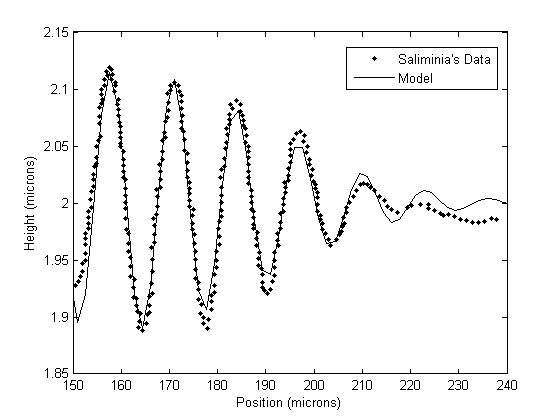
\includegraphics[width=2in]{figure/sinefigurezoom.png}
  \caption{The model's fit to a section of a surface relief profile from Saliminia's paper.}
  \label{fig:sinemodzoom}
\end{figure}

% %\begin{table}\begin{center} %\begin{tabular}{|c|c|c|c|}
%\multicolumn{4}{c}{\textbf{\Large Model Parameters for the Fit in Figure \ref{fig:sinemod}}}\\
%\hline
%\textbf{Parameter}&\textbf{Meaning}&\textbf{Fixed/Free} &\textbf{Value}\\
%\hline \hline
%$h_0$& Initial Thickness&Fixed&2 $\mu$m\\
%\hline
%$T$& Total Illumination Time&Fixed&381 s\\
%\hline
%$p_2$&Illumination Radius&Constrained&57 $\mu$m\\
%\hline
%$p_3$&Non-Oscillatory Pressure&Fixed&1\\
%\hline
%$p_4$&Frequency of Modulation&Fixed&$2\pi/13$ $\mu$m$^{-1}$\\
%\hline
%$p_5$&Modulation Phase&Fixed&$\pi/2$\\
%\hline
%$p_1/\sigma$&Relative Pressure Strength&Free&0.88 $\mu$m$^{-1}$\\
%\hline
%$\sigma/\eta$&Characteristic Growth Rate&Free&1.9$\times 10^{-3}$ $\mu$m/s\\
%\hline %\end{tabular} %\end{center} %\caption{Summary of the parameters used in
constructing the fit depicted in Figure \ref{fig:sinemod}.} %\label{tab:sinemod}
%\end{table}


\begin{table}
\begin{ruledtabular}
\begin{tabular}{l c r}
\textbf{Parameter}&\textbf{Meaning}&\textbf{Value}\\
\hline
\multicolumn{3}{c}{\textbf{Fixed Parameters}}\\
$h_0$& Initial Thickness&2 $\mu$m\\
$T$& Total Illumination Time&381 s\\
$p_2$&Illumination Radius&57 $\mu$m\\
$p_3$&Non-Oscillatory Pressure&1\\
$p_4$&Modulation Frequency&$2\pi/13$ $\mu$m$^{-1}$\\
$p_5$&Modulation Phase&$\pi/2$\\
\\
\multicolumn{3}{c}{\textbf{Free Parameters}}\\
$p_1/\sigma$&Relative Pressure Strength&0.88 $\mu$m$^{-1}$\\
$\sigma/\eta$&Characteristic Growth Rate&1.9$\times 10^{-3}$ $\mu$m/s\\
\end{tabular}
\end{ruledtabular}
\caption{Summary of the parameters used in constructing the fit depicted in Figure
\ref{fig:sinemodzoom}.} \label{tab:sinemod}
\end{table}

\begin{figure}
                                                                                                                                                                                                                                                                                                                                                                                                                                                                                                                                                                                                                                                                                                                                                                                                                                                                                                                                                                                                                                                                  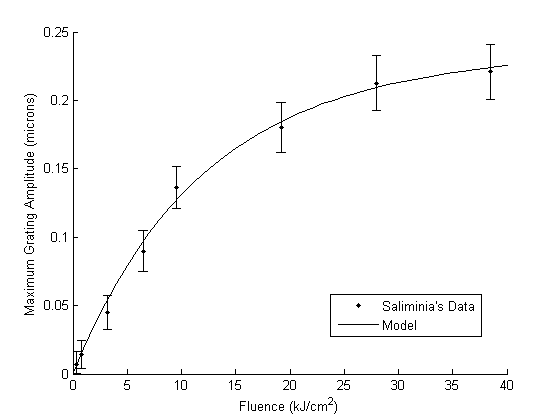
\includegraphics[width=2in]{figure/saliminiagrowth.png}
                                                                                                                                                                                                                                                                                                                                                                                                                                                                                                                                                                                                                                                                                                                                                                                                                                                                                                                                                                                                                                                                \caption{Fluence (time) dependence of maximum surface relief amplitude for the fit in Figure \ref{fig:sinemodzoom}. The $x$ axis corrects an apparent typographical error in Saliminia's original paper.}
                                                                                                                                                                                                                                                                                                                                                                                                                                                                                                                                                                                                                                                                                                                                                                                                                                                                                                                                                                                                                                                                \label{fig:salgrowth}
\end{figure}

\begin{figure}
                                                                                                                                                                                                                                                                                                                                                                                                                                                                                                                                                                                                                                                                                                                                                                                                                                                                                                                                                                                                                                                                  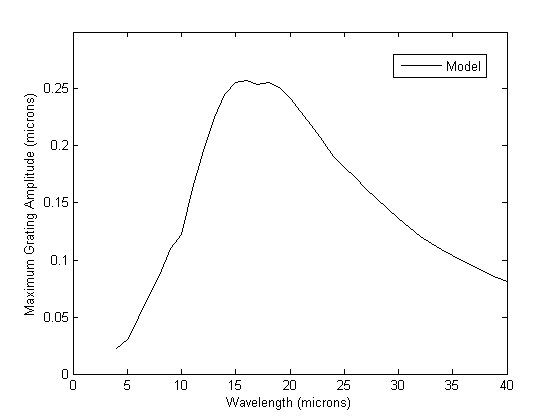
\includegraphics[width=2in]{figure/saliminiadisp.png}
                                                                                                                                                                                                                                                                                                                                                                                                                                                                                                                                                                                                                                                                                                                                                                                                                                                                                                                                                                                                                                                                \caption{Dependence of the predicted maximum surface relief amplitude on spatial modulation frequency with all other parameters as in Table \ref{tab:sinemod}. Although inconsistencies in Saliminia's reporting prevent a fit, the curve presented matches all the major qualitative features of Saliminia's graph.}
                                                                                                                                                                                                                                                                                                                                                                                                                                                                                                                                                                                                                                                                                                                                                                                                                                                                                                                                                                                                                                                                \label{fig:saldisp}
\end{figure}

\bibliography{references}% Produces the bibliography via BibTeX.

\end{document}
% % ****** End of file apssamp.tex ******
